\def \delta {0.15}

\begin{tikzpicture}
\tikzstyle{task} = [draw,thick,fill=white,align=center]

%%% TASKS %%%

\node[task,opacity=0.3] (t1) at (-1.5+0*\delta,1.6-0*\delta) {\textcolor{white}{Task $\#3$} \\\textcolor{white}{\faFileCode[regular]}};
\node[task,opacity=0.6] (t2) at (-1.5+1*\delta,1.6-1*\delta) {\textcolor{white}{Task $\#2$} \\\textcolor{white}{\faFileCode[regular]}};
\node[task,opacity=1.0] (t3) at (-1.5+2*\delta,1.6-2*\delta) {Task $\#1$ \\\faFileCode[regular]};

\node[task,opacity=0.3] (ct1) at (1+0*\delta,1.6-0*\delta) {\textcolor{white}{Control-Task $\#3$} \\\textcolor{white}{\faFileCode[regular]}};
\node[task,opacity=0.6] (ct2) at (1+1*\delta,1.6-1*\delta) {\textcolor{white}{Control-Task $\#2$} \\\textcolor{white}{\faFileCode[regular]}};
\node[task,opacity=1.0] (ct3) at (1+2*\delta,1.6-2*\delta) {Control-Task $\#1$ \\\faFileCode[regular]};

%%% CYBER %%%

\node[thick, align=center] (rtos) at (-0.1,0.25) {Real-Time Operating System};
\node[thick, draw, align=center, rotate=90, text width=2.75cm] (hw) at (3.15,0.87) {HW Interfaces};
\node[thick, fit=(rtos)(t1)(ct1)(ct3),draw,yshift=1.5mm,xshift=0.75mm] (sw) {};
\node[thick, draw, above left] (clock) at (sw.south east) {\faClock[regular]};
\node[thick, fit=(sw)(hw), inner sep=5pt, draw] (board) {};
\node[thick, above left, xshift=1.8cm] (borad-label) at (board.south west) {Board};
\node[thick, draw, above right] (clockboard) at (board.south west)  {\faClock[regular]};

%%% PHYSICAL %%%

\node[thick, draw ,align=center] (phys) at (6,0.87) {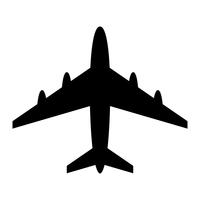
\includegraphics[scale=4]{\figdir/airplane.jpg}};
\node[thick, draw, above left] (time) at (phys.south east) {\faClock[regular]};

%%% ARROWS %%%

\draw[-latex] ([yshift=0.65cm]hw.south) to node[yshift=0.85cm,rotate=90] {Actuation} ([yshift=0.65cm]phys.west);
\draw[-latex] ([yshift=-0.65cm]phys.west) to node[yshift=-0.85cm, rotate=90] {Sensing} ([yshift=-0.65cm]hw.south);

\end{tikzpicture}
